\documentclass[pdftex,10pt,a4paper]{report}

\usepackage[pdftex]{graphicx}

\newcommand{\HRule}{\rule{\linewidth}{0.5mm}}
\usepackage{apacite}
\usepackage{fullpage}
\setcounter{tocdepth}{3}
\setcounter{secnumdepth}{0}
\usepackage{indentfirst}
\usepackage{wrapfig}
\usepackage{lipsum}
\usepackage{hyperref}
\usepackage{caption}
\usepackage{subcaption}
\hypersetup{
    colorlinks,
    citecolor=black,
    filecolor=black,
    linkcolor=black,
    urlcolor=black
}
\renewcommand{\baselinestretch}{1.5}
\makeatletter
\def\@makechapterhead#1{%
  \vspace*{50\p@}%
  {\parindent \z@ \raggedright \normalfont
    \interlinepenalty\@M
    \Huge \bfseries #1\par\nobreak
    \vskip 40\p@
  }}
  \makeatother

\begin{document}

\begin{titlepage}
\begin{center}

% Upper part of the page. The '~' is needed because \\
% only works if a paragraph has started.

\includegraphics[width=0.25\textwidth]{img/group/logo.png}~\\[1cm]

\textsc{\LARGE University of Toronto}\\[0.7cm]

\textsc{\Large CSCD01 Phase 1 Report}\\
\textsc{\large Team: Infinity}\\[0.5cm]

% Title
\HRule \\[0.4cm]
{ \huge \bfseries Reverse Engineering \\[0.4cm] }

\HRule \\[1.5cm]

% Author and supervisor
\begin{minipage}{0.4\textwidth}
\begin{flushleft} \large
Andrew \textsc{Berneshawi}\\
Nicholas \textsc{Dujay}\\
Pirave \textsc{Eahalaivan}\\
Josh \textsc{Hillen}\\
Yunqin \textsc{Huang}\\
Ho-Cheung \textsc{Lai}\\
Wei \textsc{Li}\\
Choi \textsc{Tak}\\
\end{flushleft}
\end{minipage}
\begin{minipage}{0.4\textwidth}
\begin{flushright} \large
{\tt bernesha} 998425388\\
{\tt dujaynic} 999194900\\
{\tt eahalaiv} 998152136\\
{\tt hillenjo} 999143911\\
{\tt huangy11} 996445217\\
{\tt laihoche} 999035020\\
{\tt liwei18} 999232753\\
{\tt choitak} 997905566\\
\end{flushright}
\end{minipage}

\vfill

% Bottom of the page
{\large \today}
\end{center}
\end{titlepage}

\begin{abstract}
The objective of this report is to reverse engineer a set of models from the {\tt matplotlib} source code to explain its design. The goal is to use UML to highlight the structure and behaviour of the code. The report strategically determines which aspects of the design to model, how much to abstract away from the code base, and which parts of UML to use. The models are designed to explain the most interesting and important aspects of the design.
\end{abstract}

\tableofcontents
\listoffigures

%xxxxxxxxxxxxxxxxxxxxxxxxxxxxxxxxxxxxxxxxxxxxxxxxxxxxxxxxxxx
%xxxxxxxxxxxxxxxxxxxxxxxxxxxxxxxxxxxxxxxxxxxxxxxxxxxxxxxxxxx
% BEGIN DOCUMENT
%xxxxxxxxxxxxxxxxxxxxxxxxxxxxxxxxxxxxxxxxxxxxxxxxxxxxxxxxxxx
%xxxxxxxxxxxxxxxxxxxxxxxxxxxxxxxxxxxxxxxxxxxxxxxxxxxxxxxxxxx
\chapter{Introduction}

\section{Team}

  \begin{center}
    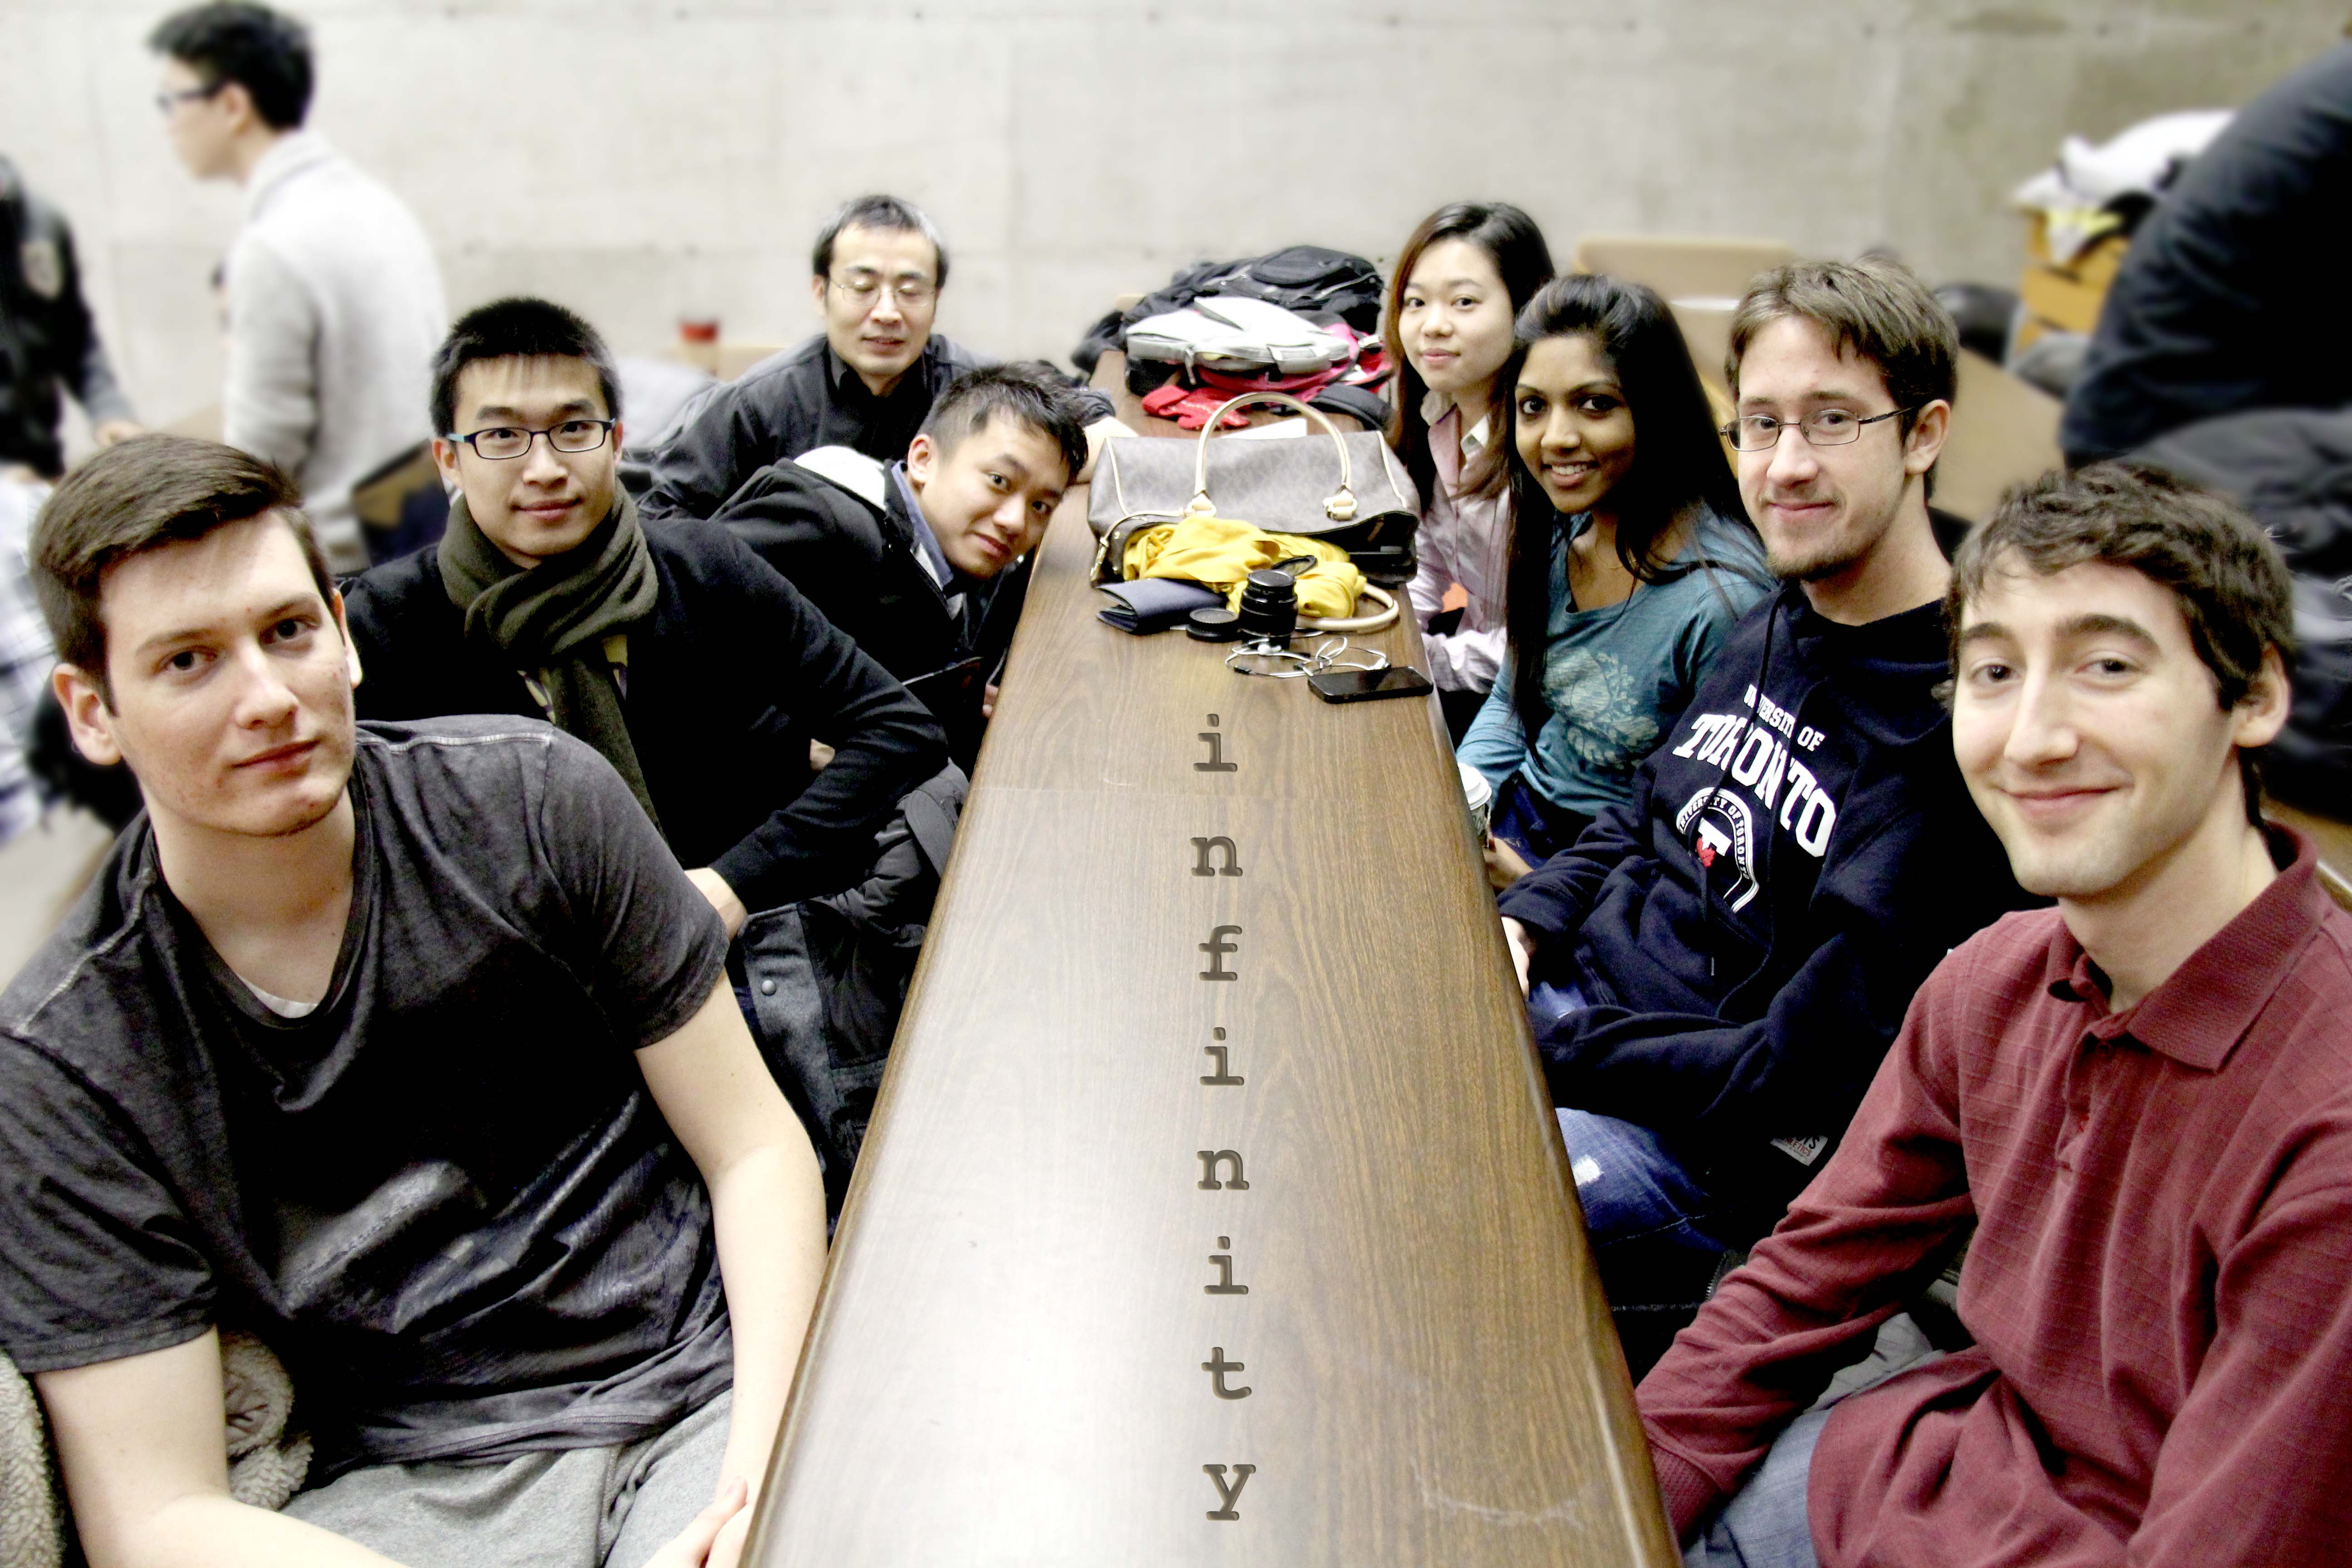
\includegraphics[width=1\textwidth]{img/group/group}
  \end{center}
We are team $\infty$.
\newpage
\section{Members}
\begin{wrapfigure}{l}{0.25\textwidth}
  \vspace{-20pt}
  \begin{center}
    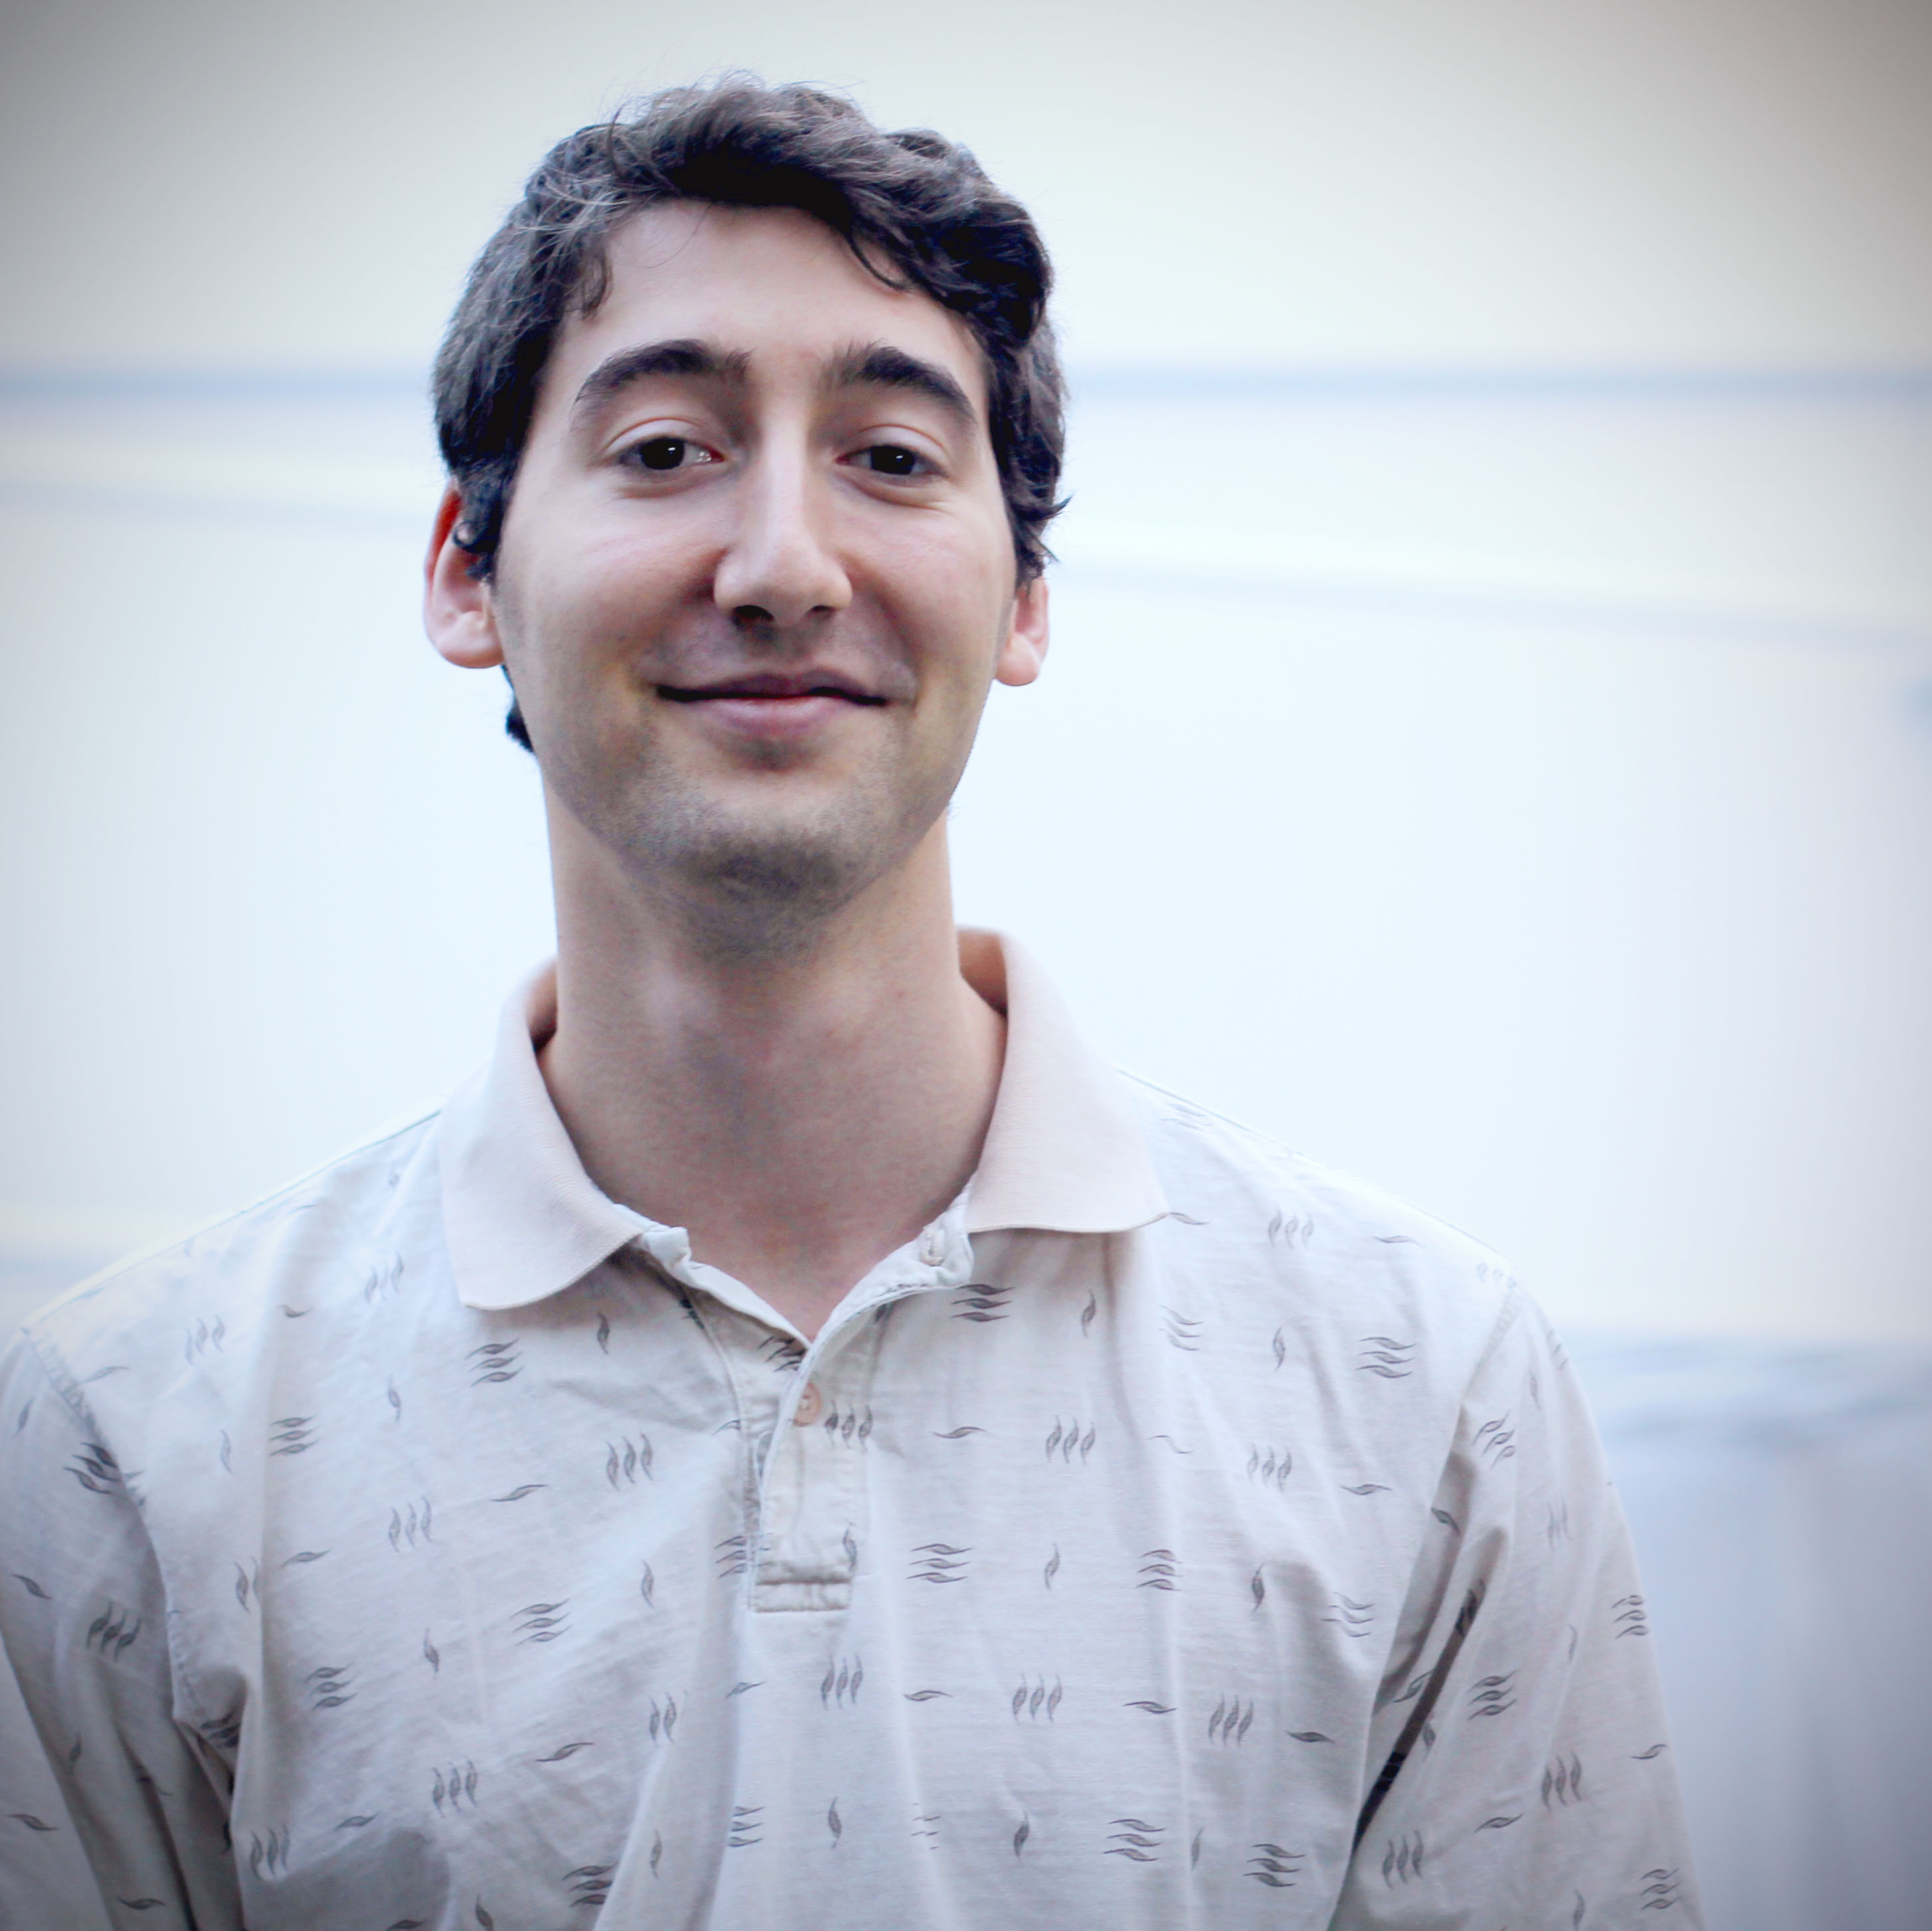
\includegraphics[width=0.25\textwidth]{img/group/andrew}
  \end{center}
  \vspace{-20pt}
\end{wrapfigure}
 Andrew Berneshawi is currently in the 3rd year of his Computer Science Specialist program in the Software Engineering stream. Thanks to his involvement in the co-op program he already has over a year of industry experience in web development. In his first internship at UTSC's IITS department he worked with PHP, followed by Java at IBM, and Java again in his latest job at Amazon; where he also gained experience with agile development. Now that he is back in class he looks forward to strengthening other parts of his software development knowledge. Not just passionate about software, Andrew also enjoys staying up to date on the latest computer hardware, and has built a few computers for his friends and himself. Outside of computer science he is interested in the sciences in general, and although the course load has been prohibitive regarding taking any challenging physics or chemistry courses, he did manage to squeeze in some psychology courses which he found very interesting. He is looking forward to using his experience from previous courses and internships to contribute to the project. \\


\begin{wrapfigure}{l}{0.25\textwidth}
  \vspace{-20pt}
  \begin{center}
    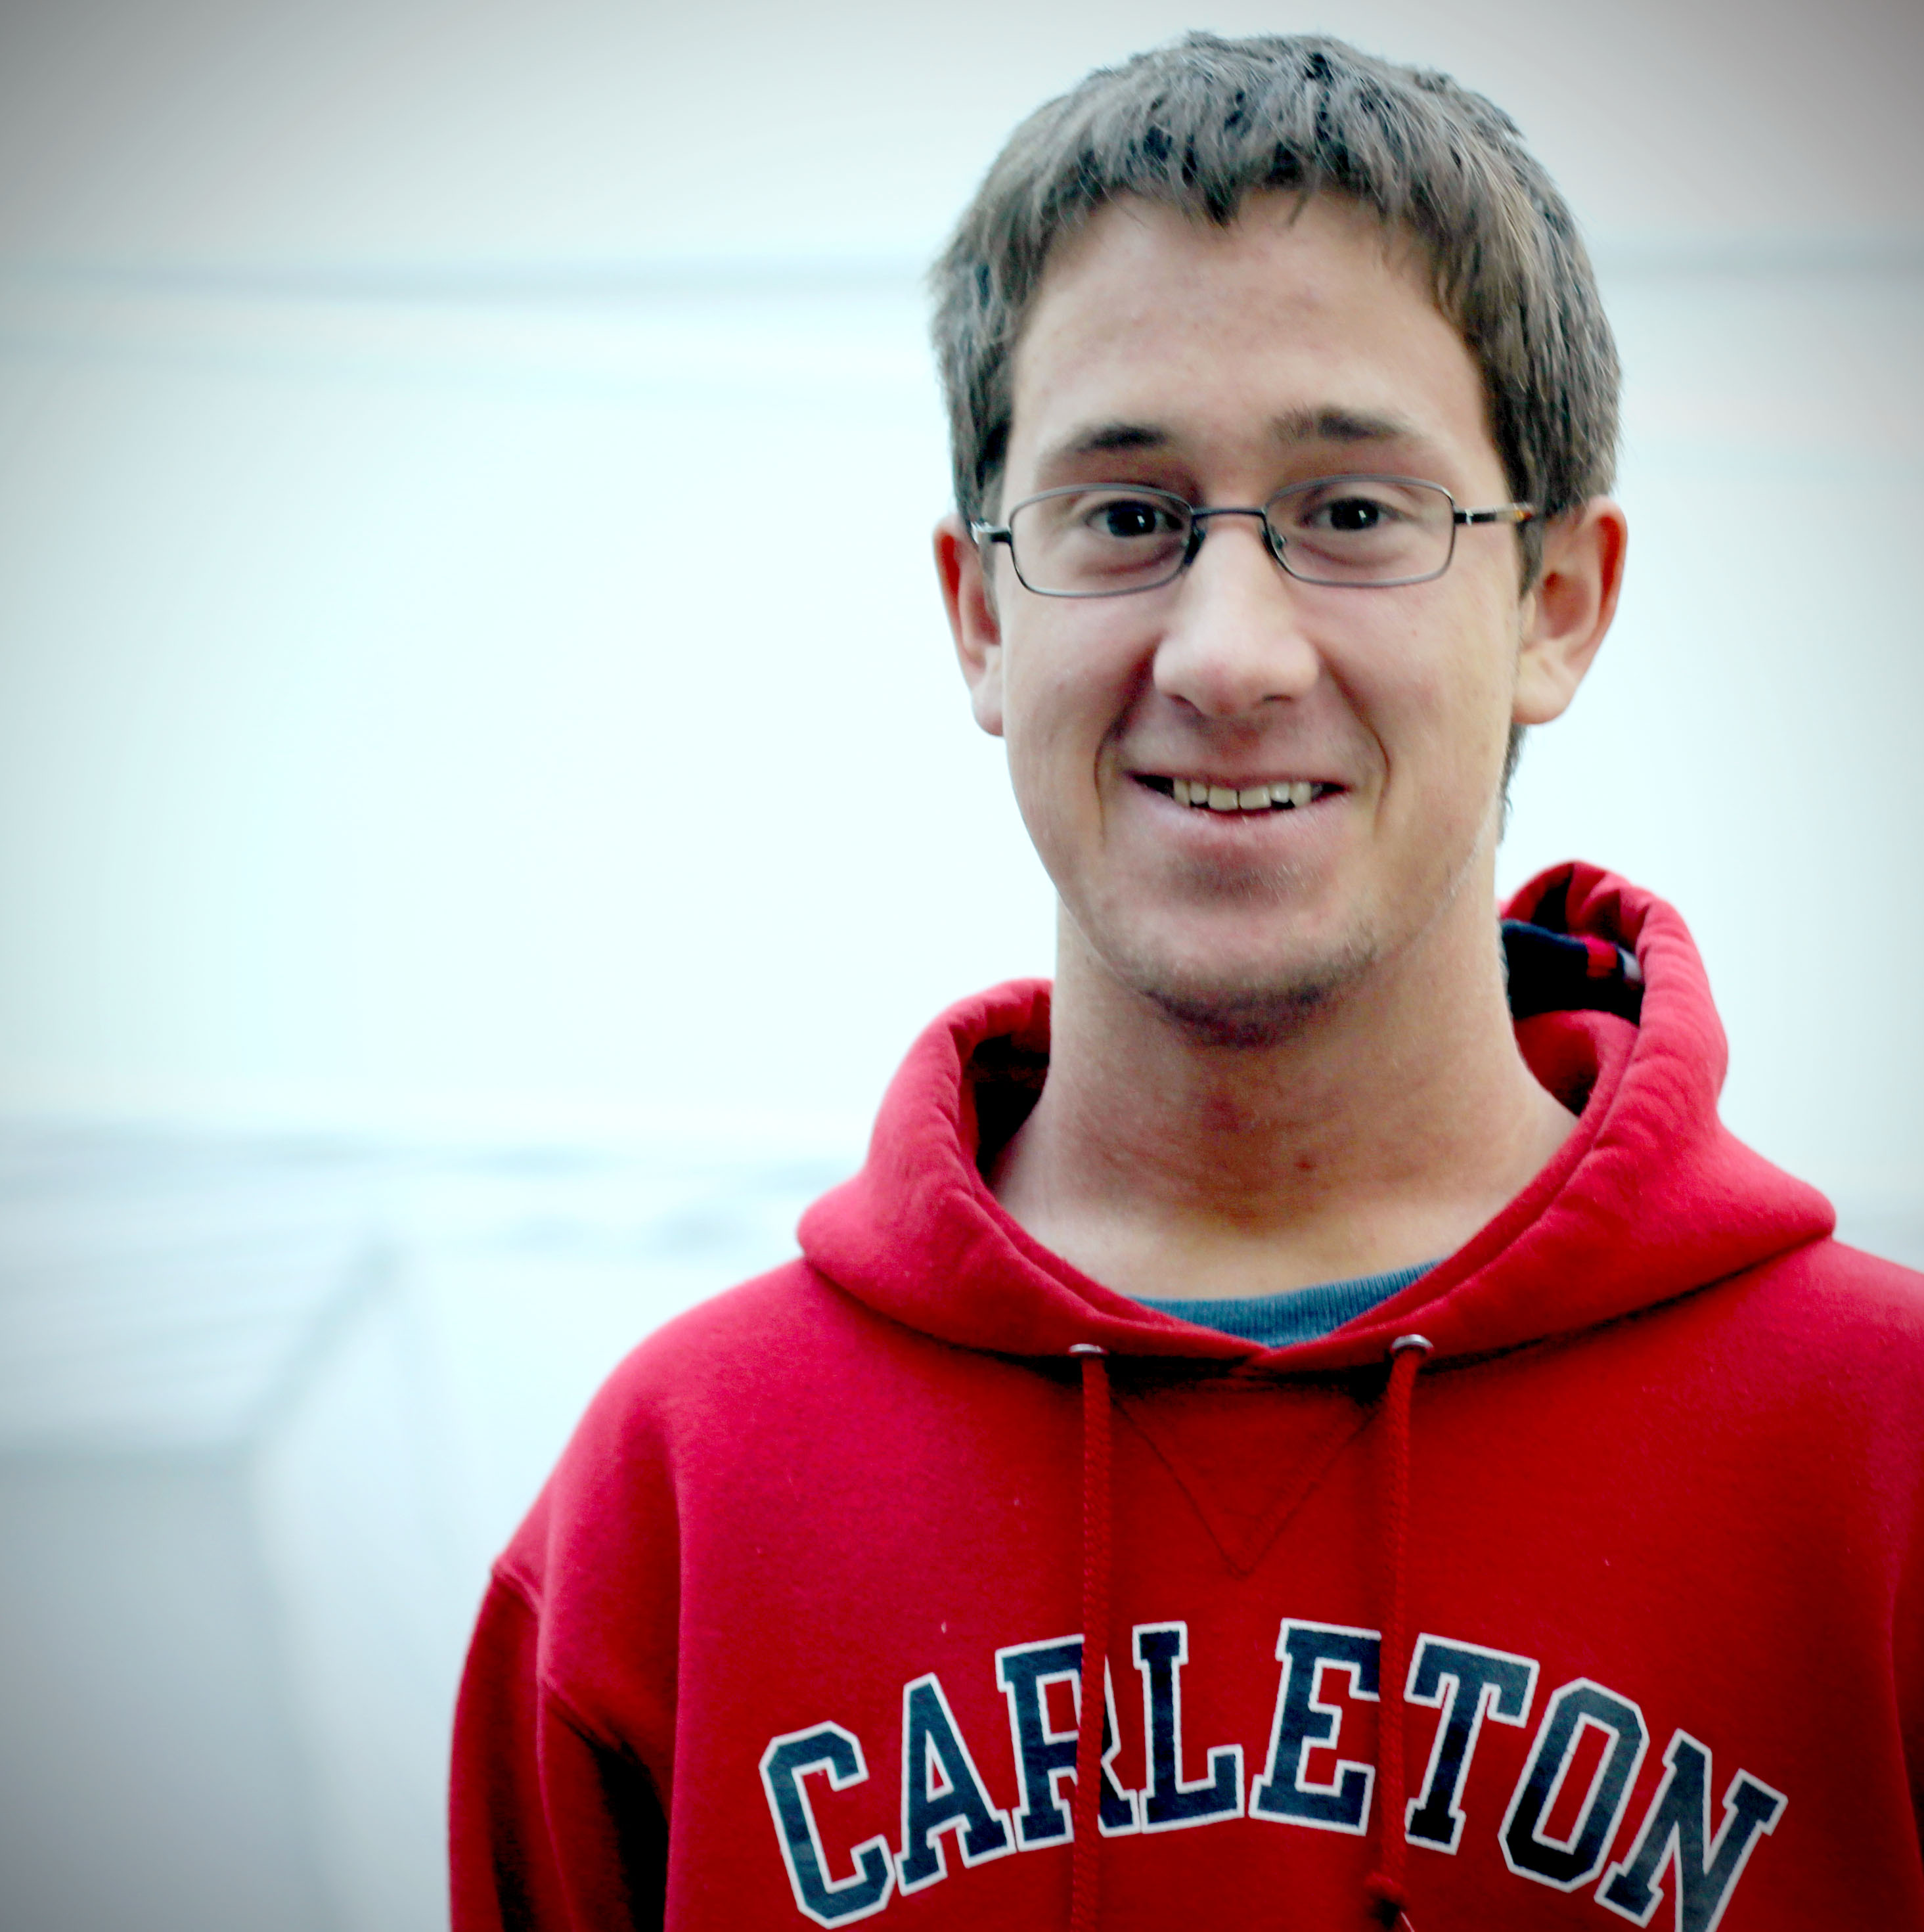
\includegraphics[width=0.25\textwidth]{img/group/nick}
  \end{center}
  \vspace{-20pt}
\end{wrapfigure}
Nicholas Dujay is a 3rd year undergraduate computer science student at the University of Toronto Scarborough Campus. He transferred from Carleton University, where he was studying to become an electrical engineer, but he decided to pursue his passion in computers and study at the University of Toronto. He is interested in learning agile, extreme programming and the software development process so he can have an idea of how software development happens in a real business setting. He is hoping to enter the video game industry after graduation, so this class will help him have an idea of how to work in a team. He spent a couple months developing a game during the summer of 2013, but had to stop development because of school. He has travelled to many places in North America, including Montreal, Moncton, New York, and Canc�n. In his spare time, he enjoys watching television shows such as Breaking Bad.\\


\begin{wrapfigure}{l}{0.25\textwidth}
  \vspace{-20pt}
  \begin{center}
    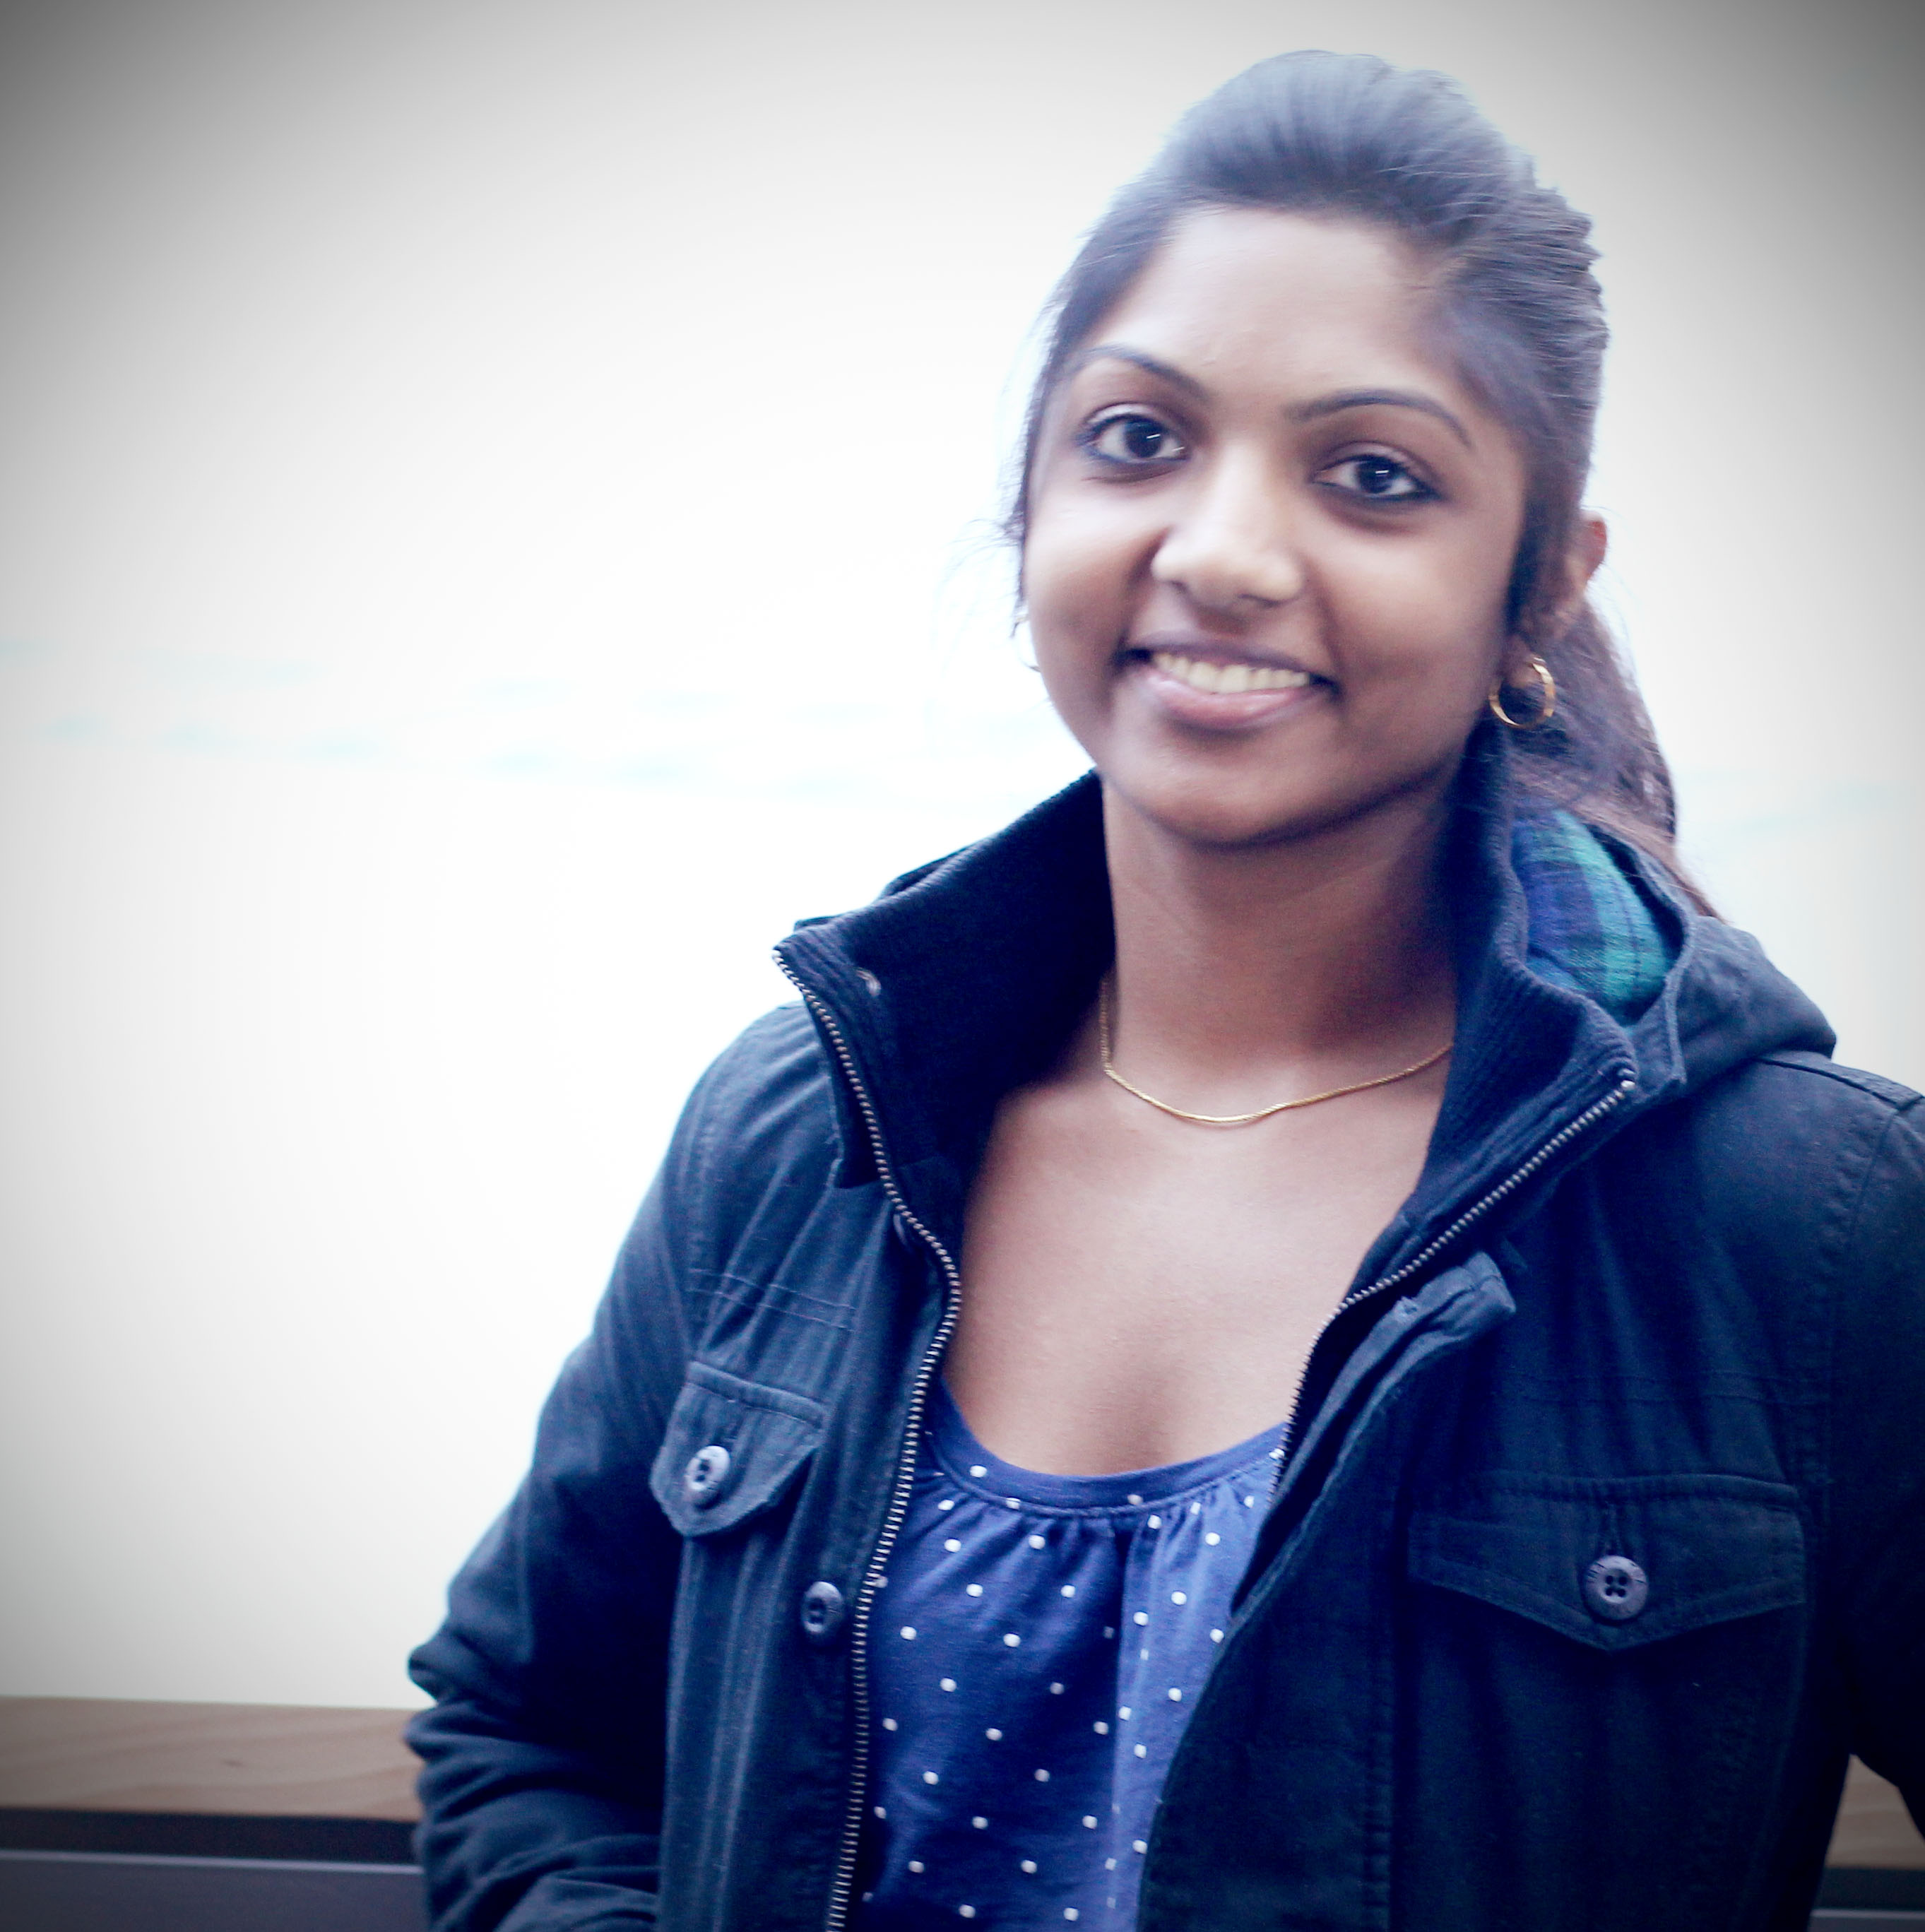
\includegraphics[width=0.25\textwidth]{img/group/pi}
  \end{center}
  \vspace{-20pt}
  \end{wrapfigure}
Pirave Eahalaivan is a 4th year student at the University of Toronto, specializing in computer science and minoring in psychology. As a part of the co-op program she has worked as a programmer analyst at Scotiabank and Ontario Teachers'Pension Plan. Her work experience has allowed her to explore web development via ASP.NET. These experiences have also enabled her to work in an agile developing environment. As the web associate for UofT's Co-op Student Association, she is responsible for designing, updating, and maintaining the club's website, using webpress. Having taken Programming on the Web (CSC309) and Databases (CSCC43), she has experience working front and back end with javascript, PHP, and MySQL. She would like to expand her horizons in web developing as well as graphic designing. She hopes to pursue a graduate degree in applied computing before she begins her career. Some of Pirave's hobbies include photography, reading and fitness.\\


\begin{wrapfigure}{l}{0.25\textwidth}
  \vspace{-20pt}
  \begin{center}
    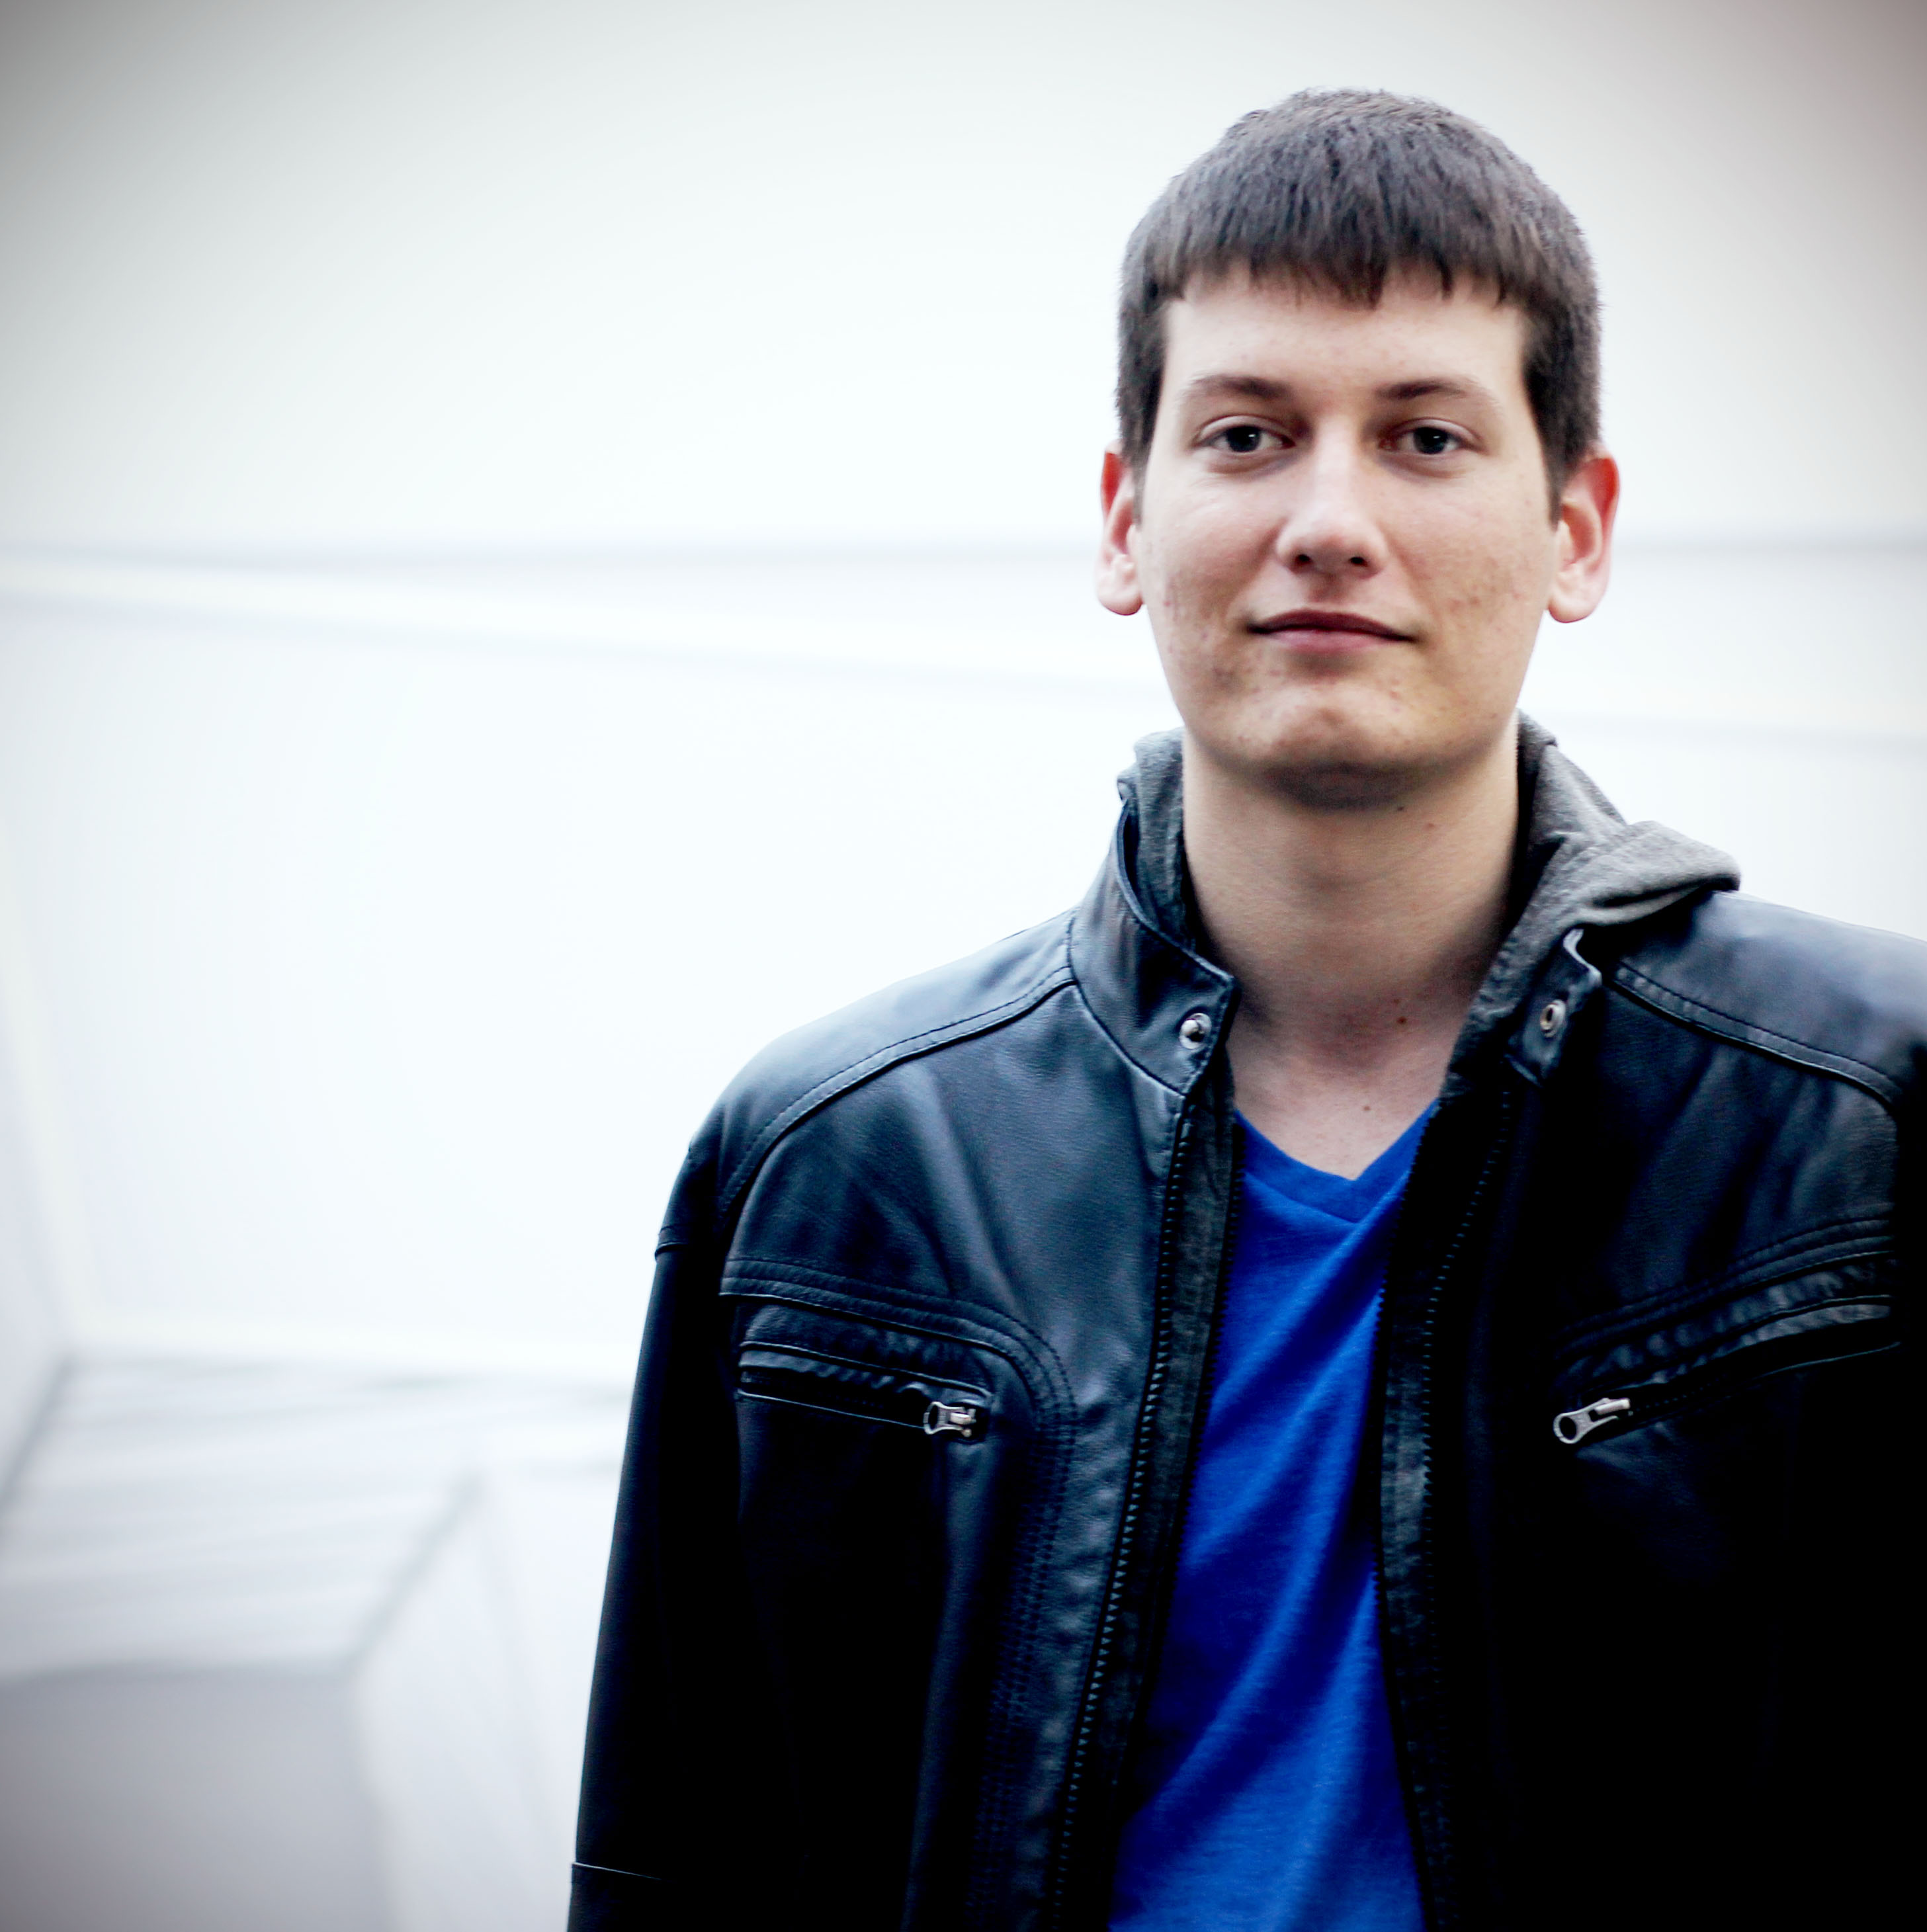
\includegraphics[width=0.25\textwidth]{img/group/josh}
  \end{center}
  \vspace{-20pt}
\end{wrapfigure}
Joshua Hillen is currently a third year student of computer science at the University of Toronto Scarborough campus. He is specializing in software engineering and plans to join the industry in 2015 directly after he graduates with an Honours Bachelor of Science. Previously to Joshua's current term he has learned and mastered a few languages, most importantly Java and C. He also participated in a group project where he was introduced to agile development and constructed software that modified .csv files for excel spreadsheets. Joshua has also taken on a variety of solo programming projects including an implementation of the Tiling Algorithm and the game Battleship. In his first two years Joshua's studies have primarily required critical thinking and time management; two important skills for group based work. He has broadened his perspective through electives including philosophy, psychology and astronomy. Joshua is a well rounded individual who has traveled overseas to Prague, Vienna, Budapest and South Africa.\\


\begin{wrapfigure}{l}{0.25\textwidth}
  \vspace{-20pt}
  \begin{center}
    
\includegraphics[width=0.25\textwidth]{default}
  \end{center}
  \vspace{-20pt}
\end{wrapfigure}
Kevin(Yunqin) Huang \lipsum[1]

\ \\
\begin{wrapfigure}{l}{0.25\textwidth}
  \vspace{-20pt}
  \begin{center}
    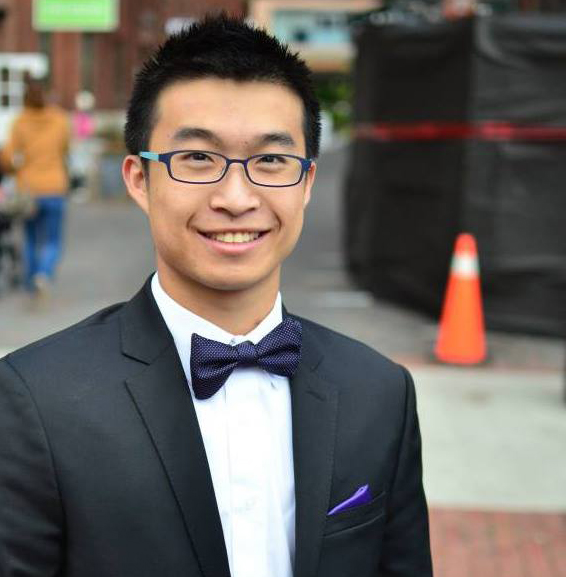
\includegraphics[width=0.25\textwidth]{img/group/derek}
  \end{center}
  \vspace{-20pt}
\end{wrapfigure}
Derek Lai was born in Hong Kong and came to Canada at the young age of 2. Ever since he was a kid, he has always wanted a job revolving around technology. Derek attended Unionville High School where he was first introduced to programming in Grade 9, learning his first programing language; Turing. From there, he furthered his computer science knowledge, learning both Visual Basic and Java. Derek is also the former President of his high school?s Robotics Team. Derek Lai is now currently a student at the University of Toronto working towards becoming a Software engineer. If not at school, he can usually be found in front of his computer or out with friends chatting over a cup of coffee.\\

\begin{wrapfigure}{l}{0.25\textwidth}
  \vspace{-20pt}
  \begin{center}
    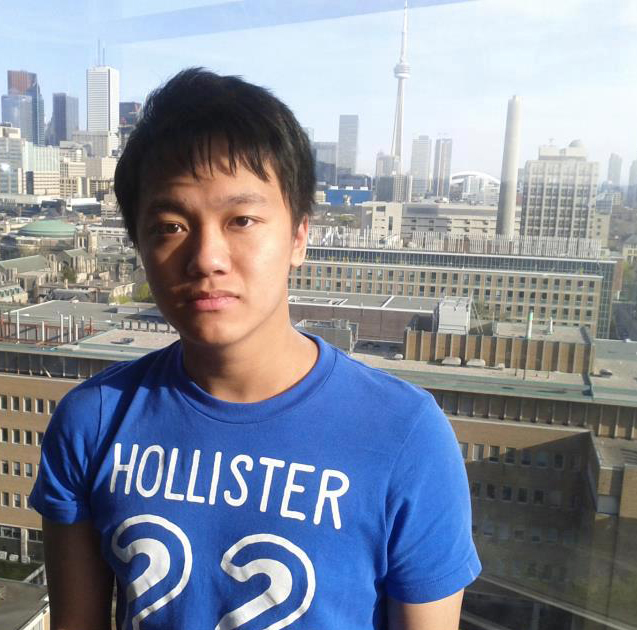
\includegraphics[width=0.25\textwidth]{img/group/dave}
  \end{center}
  \vspace{-20pt}
\end{wrapfigure}
Dave(Wei) Li \lipsum[1]


\begin{wrapfigure}{l}{0.25\textwidth}
  \vspace{-20pt}
  \begin{center}
    
\includegraphics[width=0.25\textwidth]{default}
  \end{center}
  \vspace{-20pt}
\end{wrapfigure}
Candy(Choi) Tak \lipsum[1]

\section{matplotlib}

matplotlib is a plotting library that produces quality graphics for 2D(full support) and 3D(limited support) diagrams in Python. The library is most popular in the community for Python-based scientific computing  and can be applied in many different applications. matlplotlib comes with an interactive shell that can generate figures via simple python scripts, this includes the iPython shell embded in MATLAB, IDL, or Mathematica. 

In addition, matplotlib is cross-platform compatible and can be embedded within web application servers and via any of the six GUI interface toolkits within different environments. These produce quality graphics in hardcopy that may be used for publication on the web or on paper. Supported formats include raster based graphics (PNG) and vector based graphics (PDF, PS, SVG). matplotlib can be used by a large range of users, from beginners who can use simple python commands, to power users who have full access to styling and graphical properties. A few examples of figures produced by matplotlib are illustrated in Figure~\ref{fig:examples}.

\begin{figure}
        \centering
        \begin{subfigure}[b]{0.3\textwidth}
                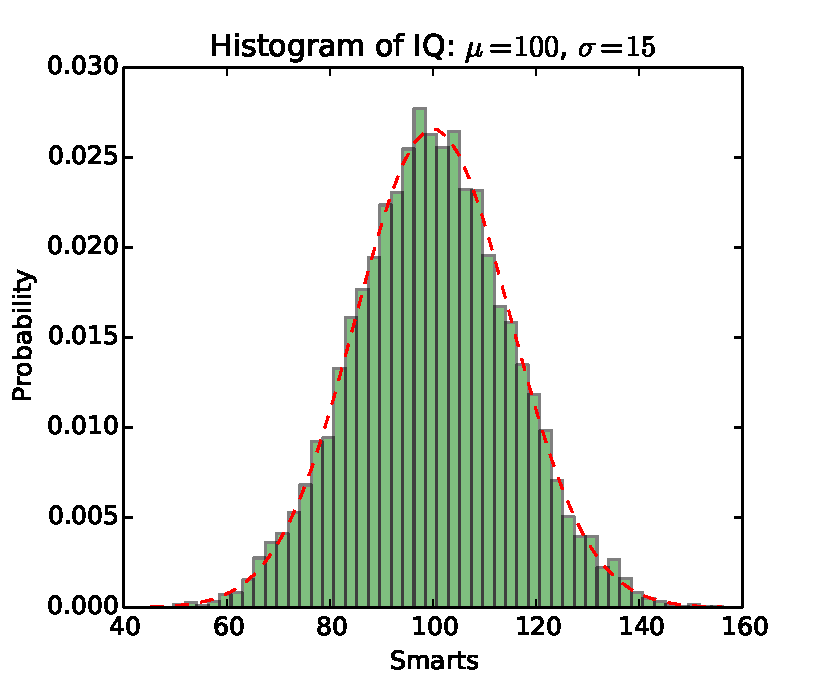
\includegraphics[width=\textwidth]{img/examples/histogram}
                \caption{Histogram example}
                \label{fig:histogram}
        \end{subfigure}%
        ~ %add desired spacing between images, e. g. ~, \quad, \qquad etc.
          %(or a blank line to force the subfigure onto a new line)
        \begin{subfigure}[b]{0.3\textwidth}
                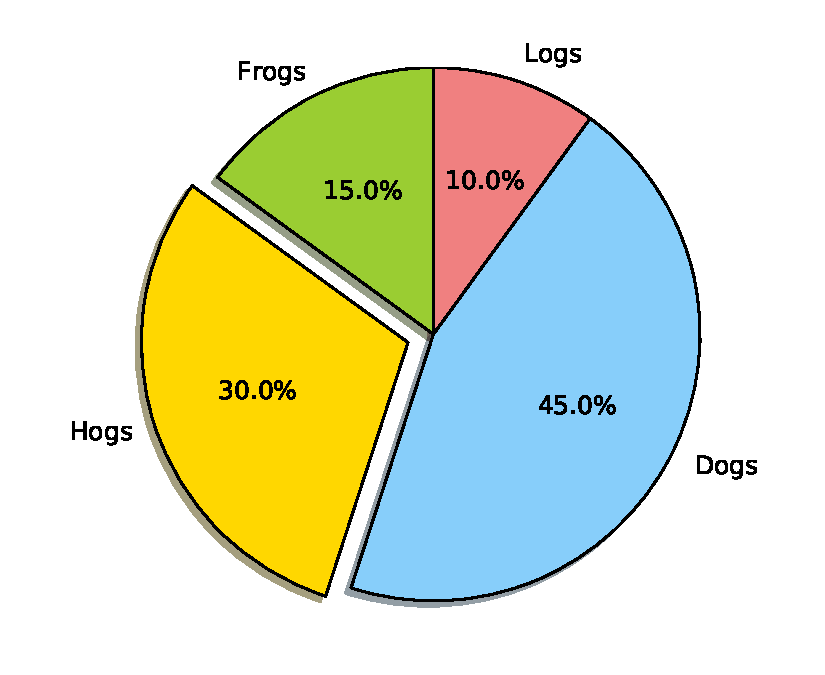
\includegraphics[width=\textwidth]{img/examples/pie}
                \caption{Pie chart example}
                \label{fig:pie}
        \end{subfigure}
        ~ %add desired spacing between images, e. g. ~, \quad, \qquad etc.
          %(or a blank line to force the subfigure onto a new line)
        \begin{subfigure}[b]{0.3\textwidth}
                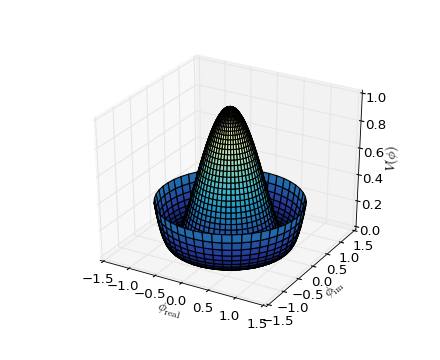
\includegraphics[width=\textwidth]{img/examples/mplot3d}
                \caption{mplot3d toolkit example}
                \label{fig:mplot3d}
        \end{subfigure}
        \caption{Examples of matplotlib graphics}\label{fig:examples}
\end{figure}



%xxxxxxxxxxxxxxxxxxxxxxxxxxxxxxxxxxxxxxxxxxxxxxxxxxxxxxxxxxx
%xxxxxxxxxxxxxxxxxxxxxxxxxxxxxxxxxxxxxxxxxxxxxxxxxxxxxxxxxxx

\chapter{The Process}

\section{Reverse Engineering Tools}

\section{Abstraction Steps}

%xxxxxxxxxxxxxxxxxxxxxxxxxxxxxxxxxxxxxxxxxxxxxxxxxxxxxxxxxxx
%xxxxxxxxxxxxxxxxxxxxxxxxxxxxxxxxxxxxxxxxxxxxxxxxxxxxxxxxxxx

\chapter{System Architecture}

%xxxxxxxxxxxxxxxxxxxxxxxxxxxxxxxxxxxxxxxxxxxxxxxxxxxxxxxxxxx
%xxxxxxxxxxxxxxxxxxxxxxxxxxxxxxxxxxxxxxxxxxxxxxxxxxxxxxxxxxx

\chapter{Chapter}
\section{Section}
\subsection{Subsection}
\subsubsection{Subsubsection}
\paragraph{Paragraph}

\begin{figure}[ht!]
\centering

\includegraphics[width=0.15\textwidth]{default}
\caption[]{Default Img}
\label{fig:overflow}
\end{figure}

blah blah blah





%xxxxxxxxxxxxxxxxxxxxxxxxxxxxxxxxxxxxxxxxxxxxxxxxxxxxxxxxxxx
%xxxxxxxxxxxxxxxxxxxxxxxxxxxxxxxxxxxxxxxxxxxxxxxxxxxxxxxxxxx
% END DOCUMENT
%xxxxxxxxxxxxxxxxxxxxxxxxxxxxxxxxxxxxxxxxxxxxxxxxxxxxxxxxxxx
%xxxxxxxxxxxxxxxxxxxxxxxxxxxxxxxxxxxxxxxxxxxxxxxxxxxxxxxxxxx

\end{document}